\chapter{基于4PCS的点云匹配算法}
\label{chap:matcher}
本章主要介绍为了估计目标的位姿所提出的一种基于4PCS的点云匹配算法A4PCS-ICP(Angle-fixed-4PCS-ICP),A4PCS-ICP主要基于全局匹配算法4PCS\cite{aiger20084}和局部匹配算法ICP\cite{besl1992method}。为了详细介绍A4PCS-ICP算法,本章首先从整体上简单介绍了A4PCS-ICP算法,包括算法所要解决的问题的具体数学描述以及相关算法的背景;然后介绍A4PCS-ICP算法的基础4PCS算法,并分析了其不足,进而提出A4PCS算法对其进行改进;接着介绍与A4PCS算法相结合的ICP算法,ICP算法主要用于提高最终点云匹配的精度;最后进行了点云匹配的实验,将本文的A4PCS-ICP算法与其他几个匹配算法相比较。

\section{点云匹配算法概述}
\subsection{问题描述}
通过第~\ref{chap:detector}~章中的目标检测算法可以得到目标的bounding box或者mask,根据bounding box或者mask可以在深度图中提取对应的区域,从而获得包含目标的点云。所以现在的问题是如何通过目标的点云计算出目标的位姿,由于可以得到目标的三维模型,因此将目标的三维模型经过一个刚体变换$T$,使之与目标点云重合,然后目标的三维模型在相机坐标系下的位姿也是已知并且可调的,为方便起见将三维模型坐标系与相机坐标系重合,则目标的位姿便等于三维模型与目标点云之间的齐次变换关系,即$T$。所以,要计算目标的位姿,就要求解目标三维模型与相机采集到的目标点云之间的刚体变换$T$,如图~\ref{fig:match_diagram}~,这也是A4PCS-ICP主要要解决的问题:两个点云之间的匹配问题。
\begin{figure}[ht]
  \centering
  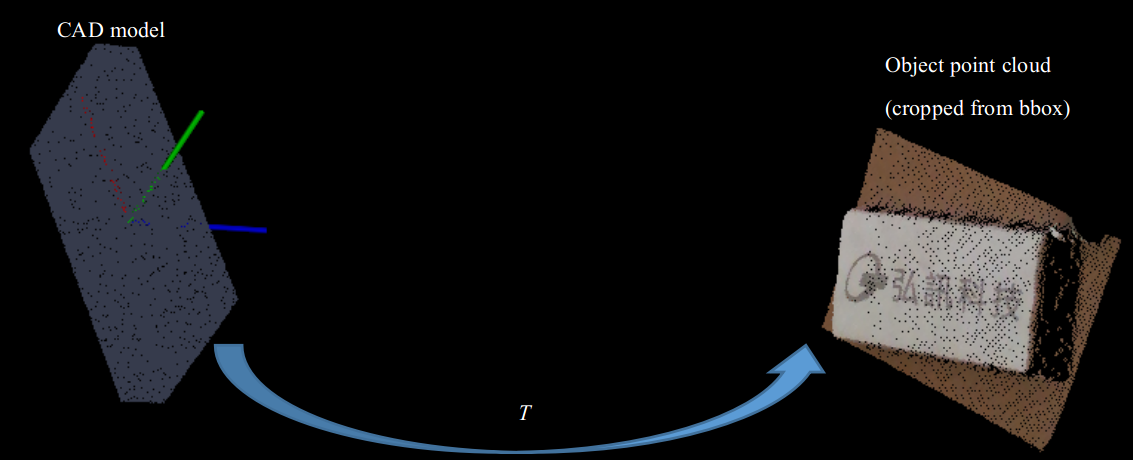
\includegraphics[width=14cm]{match_diagram}
  \caption{位姿估计示意图}
  \label{fig:match_diagram}
\end{figure}

相机所采集到的目标点云是一组包含空间三维坐标(x,y,z)以及颜色(r,g,b)的点集\footnote{对点集(point set)与点云(point cloud)不做区分,都指包含坐标点的集合},由于此处并不需要颜色信息,因此对目标点云只保留空间位置信息,去除颜色信息后的目标点云记为点集$P$。三维模型亦可通过采样得到一组包含空间三维坐标的点集,记为$Q$。A4PCS-ICP算法就可以简化为求解一个刚体变换$T$使得点集$P$中的点经过矩阵$T$变换后,尽可能与点集$Q$重合。更为准确地,A4PCS-ICP算法就可以简化为求解一个LCP(Largest Common Pointset)问题:

{\kai LCP问题:给定两个点集$P$和$Q$,在给定距离误差$\delta$下,求解点集$P$的最大子集$P'$,使得$T(P')$和点集$Q$之间的距离在合适的距离度量下小于$\delta$,其中$T$是一个刚体变换。}

\subsection{背景介绍}
LCP问题并不是一个新的问题,解决该问题的算法也有很多,尤其是近些年来,随着几何扫描相关技术的发展,如何将多次扫描或者多个设备采集的三维信息统一到一个坐标系下成为研究的热点,其本质上可以归结为LCP问题或其衍生问题,这些问题是计算机几何学和计算机视觉中的基础问题。

其中一个比较流行的算法是通过使用稳定的局部几何描述子来匹配得到粗略的刚体变换,然后紧接着使用ICP算法迭代获取较为精确的刚体变换\cite{li2005multiscale}。这种算法的效果十分取决于所选取的描述子,通常一般的描述子对传感器噪声都比较敏感,尤其是一些低精度的传感器,常用的局部几何特征描述子有SHOT\cite{salti2014shot}、FFPH\cite{rusu2009fast}等;还有一种比较流行的方法是通过几何希哈方法从事先设置好的候选集中来选择合适的刚体变换\cite{wolfson1997geometric};一些随机算法,如RANSAC(Random Sample Consesue)\cite{bolles1981ransac}通常需要足够长的时间才能保证得到合适的解。


上述介绍的一些算法,有些对噪声的鲁棒性不强,有些时间复杂度极高,有些也难以处理部分重叠的情况,即点集$P$和$Q$之间只有一部分点集是相匹配的,因此难以实际直接应用到本文所需要解决的问题,其效果也难以让人满意。对此,本文基于4PCS(4-Points Congruent Sets)算法设计了有效解决点云匹配的算法A4PCS-ICP。

\section{A4PCS-ICP算法}
\subsection{算法框架}
A4PCS-ICP算法基于4PCS,针对4PCS的瓶颈,有效地降低了其时间复杂度,然后通过与ICP算法配合提高匹配的精度,其整体框架如图~\ref{fig:4pcs-pe}~所示。
\begin{figure}[ht]
  \centering
  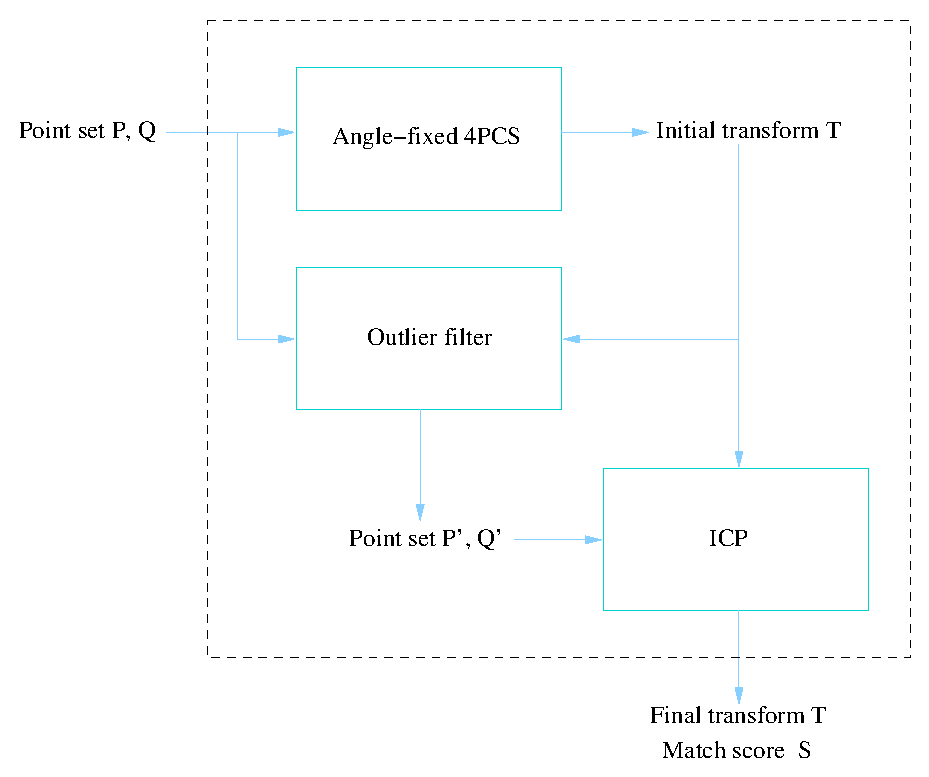
\includegraphics[width=12cm]{4pcs-pe}
  \caption{A4PCS-ICP算法框架}
  \label{fig:4pcs-pe}
\end{figure}
A4PCS-ICP由三个模块组成:Angle-fixed 4PCS、Outlier filter和ICP,Angle-fixed 4PCS是4PCS算法的优化版,也是A4PCS-ICP算法的核心,根据输入的两个点集,输出两个点集之间的粗略的变换关系;Outlier filter根据Angle-fixed 4PCS的输出对点集$P'$和$Q'$进行滤波,去掉一些离群点,用以提高下一步ICP算法的精度;ICP模块通过以Angle-fixed filter输出的变换关系为初始值对滤波后的两个点集进行迭代求解最佳的刚体变换关系,输出最终的变换关系$T$和匹配的分数$S$,$T$也是目标的位姿,$S$是点云匹配误差的倒数,实验部分会具体介绍匹配误差。

\subsection{Angle-fixed 4PCS算法}
介绍Angle-fixed 4PCS算法之前,首先先详细介绍一下4PCS算法,4PCS算法是一个对3D点集全局匹配的算法,即使所给的两个3D点集有小的重叠,4PCS都能给出较好的结果,并且对噪声有一定的鲁棒性。这种方法对初始位姿没有任何要求,其核心是从3D点集中提取出所有与给定平面4-points近似全等的共面4-points,该算法时间复杂度为$O(n^2+k)$,其中$n$是3D点集中点的个数,$k$是提取出的4-points个数。4PCS使用十分广泛,并且引申出许多相关的变种\cite{corsini2013fully}。

\begin{algorithm}
  \caption{4PCS算法}
  \label{alg:4pcs}
  \KwIn{Point sets $P$ and $Q$, measure level $\delta$}
  \KwOut{Rigid transform $T$}
  $h\leftarrow 0$\;
  \For {$i = 1$ to $L$} {
    $B\leftarrow$ SELECTCOPLANARBASE($P$)\;
    $U\leftarrow$ FINDCONGRUENT($B,Q,\delta$)\;
    \ForAll {4-points coplannar sets $U_i\in U$} {
      $T_i\leftarrow$ best rigid transform that aligns $B$ to $U_i$ in the least square sense\;
      Find $S_i\subseteq P$, such that $d(T_i(S_i), Q)\leq\delta$\;
    }
    $k\leftarrow arg\;\underset{i}{max}\left\{|S_i|\right\}$\;
    \If {$|S_k| > h$} {
      $h\leftarrow |S_k|$\;
      $T\leftarrow T_k$\;
    }
    \Return $T$\;
  }
  \BlankLine
  \BlankLine
  \BlankLine
  \BlankLine
  \SetKwProg{Def}{def}{:}{}
  \Def{FINDCONGRUENT($B:=\left\{\mathbf{b}_1,\mathbf{b}_2,\mathbf{b}_3,\mathbf{b}_4\right\},Q,\delta)$} {
    $d_1\leftarrow\;\parallel\mathbf{b}_1-\mathbf{b}_2\parallel$\;
    $d_2\leftarrow\;\parallel\mathbf{b}_3-\mathbf{b}_4\parallel$\;
    计算$R_1\equiv\left\{(\mathbf{p}_i,\mathbf{p}_j)\;|\;\mathbf{p}_i,\mathbf{p}_j\;\in Q\right\}$,使得$\parallel\mathbf{p}_i-\mathbf{p}_j\parallel\;\in [d_1-\delta,d_1+\delta]$\;
    计算$R_2\equiv\left\{(\mathbf{p}_i,\mathbf{p}_j)\;|\;\mathbf{p}_i,\mathbf{p}_j\;\in Q\right\}$,使得$\parallel\mathbf{p}_i-\mathbf{p}_j\parallel\;\in [d_2-\delta,d_2+\delta]$\;
    \ForAll {$r_{1i}\in R_1$} {
      计算与定量$r_1$和$r_2$相关的四个点$\left\{\mathbf{e}_{1i}^1,\mathbf{e}_{1i}^2,\mathbf{e}_{1i}^3,\mathbf{e}_{1i}^4\right\}$,记$\Pi(\mathbf{e}_{1i}^j)=r_{1i}$\;
    }
    对点集$\left\{\mathbf{e}_{1i}^j\right\}$在$\mathbb{R}^3$空间建立range tree的数据结构\;
    \ForAll {$r_{2i}\in R_1$} {
      计算与定量$r_1$和$r_2$相关的四个点$\left\{\mathbf{e}_{2i}^1,\mathbf{e}_{2i}^2,\mathbf{e}_{2i}^3,\mathbf{e}_{2i}^4\right\}$,记$\Pi(\mathbf{e}_{1i}^j)=r_{1i}$\;
    }
    $U'\leftarrow\varnothing$\;
    \ForAll {$\mathbf{e}_{2i}^j$} {
      在range tree中以$\delta$为领域检索点$\mathbf{e}_{2i}^j$附近的点,对于每个检索到的点$\mathbf{q}$,建立与$B$相对应的4个点的点集$U'\leftarrow\left\{U',(\Pi(\mathbf{q}),\Pi(\mathbf{e}_{2i}^j))\right\}$\;
    }
    \Return $U'$\;
  }
\end{algorithm}

{\kai 4PCS算法流程}:算法流程如\ref{alg:4pcs}所示,该算法输入两个点集$P$和$Q$,还有距离参数$\delta$,返回两个点集之间的刚体变换$T$。4PCS基于以下事实:{\kai 共面点集中定义的比例在仿射变换,包括刚体运动中保持不变。}举例来说,定义点集$X:=\left\{\mathbf{a},\mathbf{b},\mathbf{c},\mathbf{d}\right\}$,其中4个点不都在同一条直线上,设直线$ab$和$cd$相交于点$\mathbf{e}$,定义两个比例:
\begin{equation}
  \begin{array}{ccc}
    r_1& =& {\parallel \mathbf{a}-\mathbf{e}\parallel}/{\parallel \mathbf{a}-\mathbf{b}\parallel}\\
    r_2& =& {\parallel \mathbf{c}-\mathbf{e}\parallel}/{\parallel \mathbf{c}-\mathbf{d}\parallel}
  \end{array}
\end{equation}
则在仿射变换下所定义的$r_1$和$r_2$均保持不变,如图\ref{fig:4points}。
\begin{figure}[ht]
  \centering
  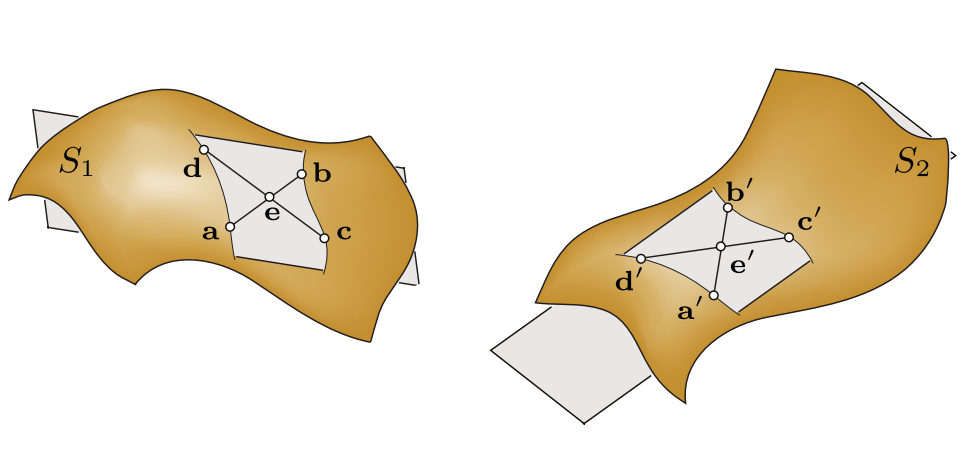
\includegraphics[width=12cm]{4points}
  \caption{4-points比例的仿射不变性}
  \label{fig:4points}
\end{figure}
如果曲面$S_1$和$S_2$匹配,并且4-points共面基在重叠区域,则$\mathbf{a},\mathbf{b},\mathbf{c},\mathbf{d}$对应的四个点$\mathbf{a}',\mathbf{b}',\mathbf{c}',\mathbf{d}'$也共面,并且
\begin{equation}
  \begin{array}{ccc}
    {\parallel \mathbf{a}'-\mathbf{e}'\parallel}/{\parallel \mathbf{a}'-\mathbf{b}'\parallel}&=&r_1\\
    {\parallel \mathbf{c}'-\mathbf{e}'\parallel}/{\parallel \mathbf{c}'-\mathbf{d}'\parallel}&=&r_2\\
  \end{array}
\end{equation}


4PCS算法另一个关键技术是使用了{\kai 宽基}(\emph{wide-base}),相比于一般的基,宽基中基的长度更长,如图\ref{fig:wide-base}所示,图片上半部分是使用宽基匹配的曲线,图片下半部分是使用一般的基匹配的曲线,显然,通过比较可以发现宽基相比普通基有更稳定的匹配结果,相关理论证明见文献\cite{goodrich1994practical}。
\begin{figure}[ht]
  \centering
  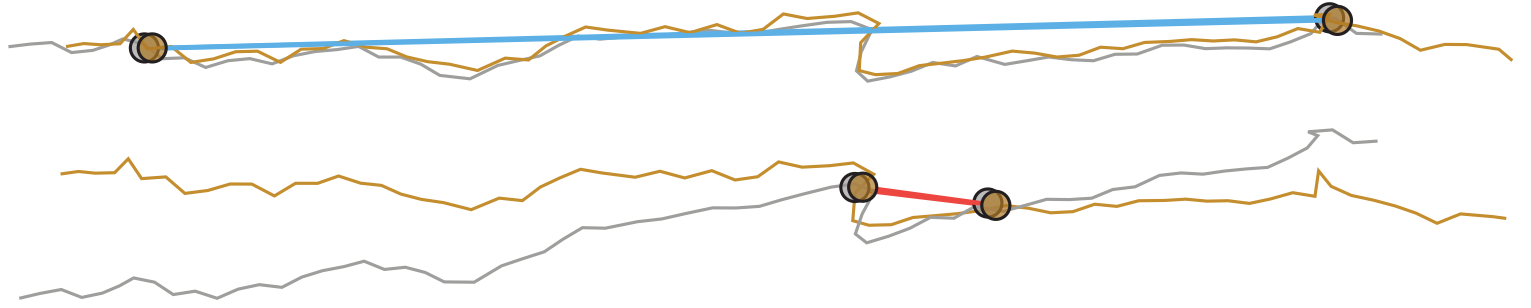
\includegraphics[width=14cm]{wide-base}
  \caption{宽基的匹配稳定性}
  \label{fig:wide-base}
\end{figure}

回到4PCS算法具体实现,算法的主体其实是一个RANSAC循环,每次循环首先会从点集$P$中挑选共面的宽基$B$,具体实现时,先从点集$P$中随机选取3个点,然后在剩下的点中选取第四个点构成共面的四点,第四个点的选取尽可能使得每个点之间的距离最大(因为我们要使用宽基),并且与前3个点近似共面(显然由于噪声的存在,完全共面并不现实),但如果第四个点选取的过远也会出现问题,因为如果宽基超过两个点集的重叠区域则难以匹配,因此当选以最大距离取宽基造成误差变大时以$f=1,0.5,0.25,\ldots$的比率降低最大距离来选取宽基。

在点集$P$中选取好宽基$B$后,算法下一步会在点集$Q$中通过4-points的仿射不变性找出所有与宽基$B$“全等”的基,构成集合$U$。在$Q$中选取基的方法见算法\ref{alg:4pcs}中的FINDCONGRUENT函数,函数首先使用基$B$中的点先定义两个仿射无关的比例,如图\ref{fig:findbase}中左边的图所示。
\begin{figure}[ht]
  \centering
  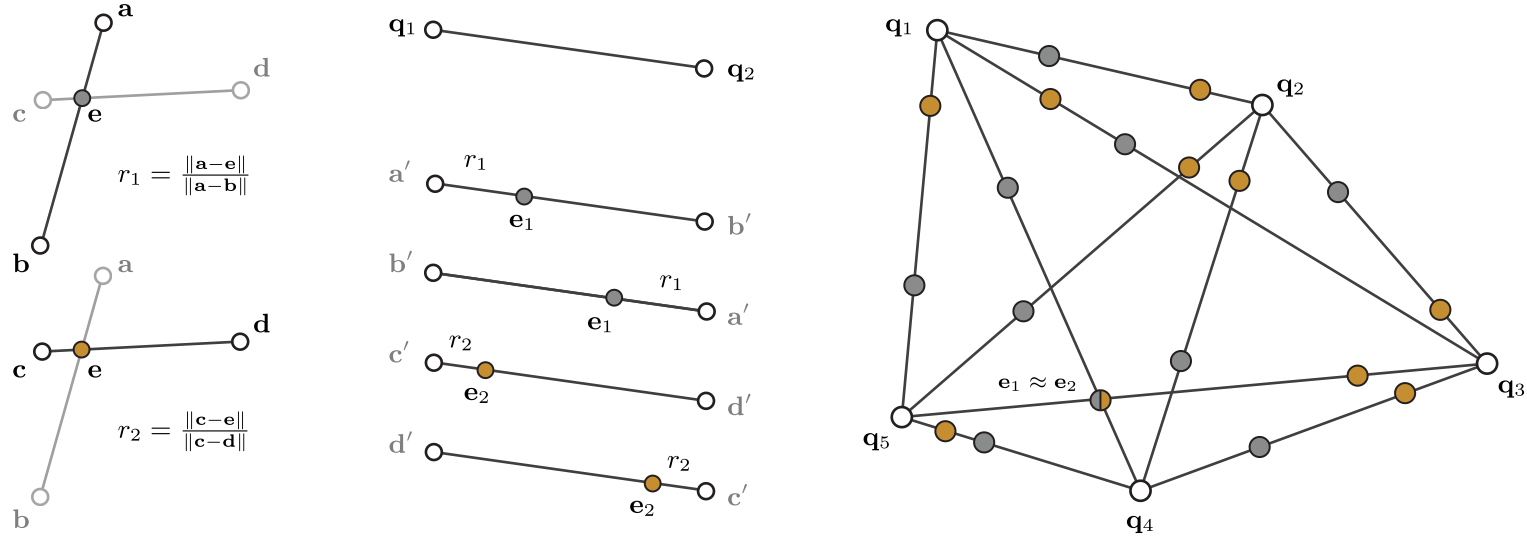
\includegraphics[width=15cm]{findbase}
  \caption{寻找近似“全等”的基示意图}
  \label{fig:findbase}
\end{figure}
假设在点集$Q$中找到两点$\mathbf{q}_1$和$\mathbf{q}_2$,并且$\left|\parallel \mathbf{q}_1-\mathbf{q}_2\parallel - \parallel \mathbf{a}-\mathbf{b}\parallel\right| \leq \delta$,则点$\mathbf{q}_1,\mathbf{q}_2$有可能与点$\mathbf{a}, \mathbf{b}$对应,则直线$\mathbf{a}\mathbf{b}$与$\mathbf{c}\mathbf{d}$相交的点$\mathbf{e}$的对应点可能为
\begin{equation}
  \mathbf{e}_1 = \mathbf{q}_1 + r1(\mathbf{q}_2-\mathbf{q}_1)
\end{equation}
或者
\begin{equation}
  \mathbf{e}_1 = \mathbf{q}_2 + r1(\mathbf{q}_1-\mathbf{q}_2)
\end{equation}
同理也可以根据$\mathbf{c},\mathbf{d}$的对应点(设为$\mathbf{q}_3, \mathbf{q}_4$)求得$\mathbf{e}$的对应点
\begin{equation}
  \mathbf{e}_2 = \mathbf{q}_3 + r1(\mathbf{q}_4-\mathbf{q}_3)
\end{equation}
或者
\begin{equation}
  \mathbf{e}_2 = \mathbf{q}_4 + r1(\mathbf{q}_3-\mathbf{q}_4)
\end{equation}
则当$\mathbf{e}_1\approx \mathbf{e}_2$时,$\mathbf{q}_1,\mathbf{q}_2,\mathbf{q}_3,\mathbf{q}_4$就是我们所要找的一组与点$\mathbf{a},\mathbf{b},\mathbf{c},\mathbf{d}$近似“全等”的基,如图\ref{fig:findbase}中右边图中的$\mathbf{q}_5,\mathbf{q}_3,\mathbf{q}_4,\mathbf{q}_1$。

具体实现时,当我们在点集$Q$中找出了所有可能的$\mathbf{e}_1$和$\mathbf{e}_2$后,找出其中近似相等的$\mathbf{e}_1$和$\mathbf{e}_2$可以通过range树\cite{arya1998optimal}来实现,对于大小为$n$的点集,range树的建立时间复杂度为$O(n\lg n)$,查询附近点的时间复杂度为$O(\lg n + k)$,其中$k$是查询到点的个数。

在$Q$中找出所有与基$B$近似“全等”的基后,下一步就是计算出最优的刚体变换$T$。对于$U$中的每个基$U_i$,我们可以利用最小二乘\cite{horn1987closed}的思想计算$B$到$U_i$的刚体变换$T_i$。得到刚体变换$T_i$后,我们将点集$P$进行变换$T_i$,然后对变换后的点集中的点在$Q$中查找最近点,统计最近点距离小于$\delta$的个数$S_i$,$S_i$也是评价$T_i$效果的分数,分数越高的$T_i$就是我们要求的最优刚体变换$T$。

{\kai 4PCS算法时间复杂度:}设输入的两个点集$P,Q$的大小分别为$m,n$。算法中最耗时的部分是FINDCONGRUENT函数:从点集$Q$中选取距离为$d_1$和$d_2$的点对,其时间复杂度为$O(n^21)$,然后建立和查询range树,其复杂度为$O(n^2+k$,其中$k$是满足条件的基个数,因此4PCS算法整体的时间复杂度为$O(n^2+k)$,空间复杂度显然为$O(n)$。

{\kai 4PCS算法不足:}仔细研究4PCS算法,可以发现从点集$Q$中提取的基与$B$并不是全等的,如图\ref{fig:4pcs-flaw}所示,
\begin{figure}[ht]
  \centering
  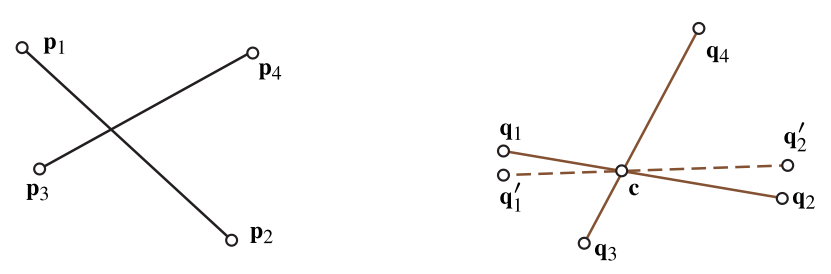
\includegraphics[width=12cm]{4pcs-flaw}
  \caption{4PCS中"全等“的基}
  \label{fig:4pcs-flaw}
\end{figure}
将线段$\mathbf{q}_1\mathbf{q}_2$绕交点转动一定角度后便不再与原基全等,但是4PCS仍然会找出点$\mathbf{q}_1',\mathbf{q}_2',\mathbf{q}_3,\mathbf{q}_4$作为与$\mathbf{p}_1',\mathbf{p}_2',\mathbf{p}_3,\mathbf{p}_4$全等的基。这一缺点会导致4PCS算法需要更多的求解时间,并且还有可能影响最终的匹配结果。因此,对4PCS改进去除这些与原基不是全等的基很有必要。改进后的算法如算法\ref{alg:a4pcs}所示,滤去不全等的基的算见其中的FILTERCONGRUENT函数。
\begin{algorithm}
  \caption{A4PCS算法}
  \label{alg:a4pcs}
  \KwIn{Point sets $P$ and $Q$, distance tolerance $\delta$, angle tolerance $\epsilon$}
  \KwOut{Rigid transform $T$}
  $h\leftarrow 0$\;
  \For {$i = 1$ to $L$} {
    $B\leftarrow$ SELECTCOPLANARBASE($P$)\;
    $U\leftarrow$ FINDCONGRUENT($B,Q,\delta$)\;
    $U\leftarrow$ FILTERCONGRUENT($B,U,\epsilon$)\;
    \ForAll {4-points coplannar sets $U_i\in U$} {
      $T_i\leftarrow$ best rigid transform that aligns $B$ to $U_i$ in the least square sense\;
      Find $S_i\subseteq P$, such that $d(T_i(S_i), Q)\leq\delta$\;
    }
    $k\leftarrow arg\;\underset{i}{max}\left\{|S_i|\right\}$\;
    \If {$|S_k| > h$} {
      $h\leftarrow |S_k|$\;
      $T\leftarrow T_k$\;
    }
    \Return $T$\;
  }
  \BlankLine
  \BlankLine
  \BlankLine
  \BlankLine
  \SetKwProg{Def}{def}{:}{}
  \Def{FILTERCONGRUENT($B:=\left\{\mathbf{b}_1,\mathbf{b}_2,\mathbf{b}_3,\mathbf{b}_4\right\},U,\epsilon)$} {
    $U'\leftarrow \varnothing$\;
    $a\leftarrow \overrightarrow{\mathbf{b}_1\mathbf{b}_2}\cdot \overrightarrow{\mathbf{b}_3\mathbf{b}_4}$\;
    \ForAll {$U_i:=\left\{\mathbf{q}_1,\mathbf{q}_2,\mathbf{q}_3,\mathbf{q}_4\right\}\in U$} {
      $a'\leftarrow \overrightarrow{\mathbf{q}_1\mathbf{q}_2}\cdot \overrightarrow{\mathbf{q}_3\mathbf{q}_4}$\;
      \If {$a'\in [a-\epsilon,a+\epsilon]\cup [-a-\epsilon,-a+\epsilon]$} {
        $U'\leftarrow \left\{U',U_i\right\}$\;
      }
    }
    \Return $U'$\;
  }
\end{algorithm}

\subsection{Outlier filter}
从图~\ref{fig:match_diagram}其实可以看出目标点云有许多点并不属于目标物体,尤其是检测结果没有mask只能使用bbox分割目标时,不属于目标物体的离群点就尤其的多。因此,为了提高最终的匹配精度,除去这些离群点十分有必要,Outlier filter模块的作用就是根据Angle-fixed 4PCS输出的初始刚体变换来去除点云数据中的离群点,从而提升下一步ICP算法匹配的精度,使最终估计的位姿精度提高。

Outlier filter模块的核心算法如算法\ref{alg:outlier-filter}所示。
\begin{algorithm}[ht]
  \caption{Outlier filter算法}
  \label{alg:outlier-filter}
  \KwIn{Point sets $P$ and $Q$, Initial transform $T$, Distance tolerance $\delta$}
  \KwOut{Point sets $P'$ and $Q'$}
  $P'\leftarrow P$\;
  $Q'\leftarrow \varnothing$\;
  \ForAll {point $\mathbf{p}_i\in P$} {
    $\mathbf{p}_i\leftarrow T(\mathbf{p}_i)$\;
  }
  对点集$P$在$\mathbb{R}^3$空间建立kd树的数据结构\;
  \ForAll {point $\mathbf{q}_i\in Q$} {
    在kd树中检索出距离点$\mathbf{q}_i$最近的点$\mathbf{p}$\;
    $d\leftarrow\;\parallel\mathbf{q}_i-\mathbf{p}\parallel$\;
    \If {$d \leq \delta$} {
      $Q'\leftarrow \left\{Q', \mathbf{q}_i\right\}$\;
    }
  }
  \Return $P'$,$Q'$\;
\end{algorithm}
算法输入点集$P$和$Q$,需要参数初始刚体变换$T$,以及允许的距离误差$\delta$,由于点集$P$是由物体的CAD模型转换过来的,因此不对其进行滤波,只对点集$Q$进行离群点去除。具体方法是,首先使用$T$对点集$P$进行刚体变换;然后对变换后的点集建立kd树,建立kd树的目的是为了快速在点集$P$中找到距离某点最近的点,其查找的时间复杂度为$O(kN^{1-1/k}$,其中$k$是所建立kd树的维数,显然对于三维空间中点集为3,$N$是建立的kd树的节点个数;建立好kd树后,对点集$Q$中的每个点在kd树中找到与之距离最近的点,如果两点间的距离大于所设的参数$\delta$,则在点集Q中去除该点。实际运行Outlier filter算法的效果如图\ref{fig:outlier-filter}所示。
\begin{figure}[ht]
  \centering
  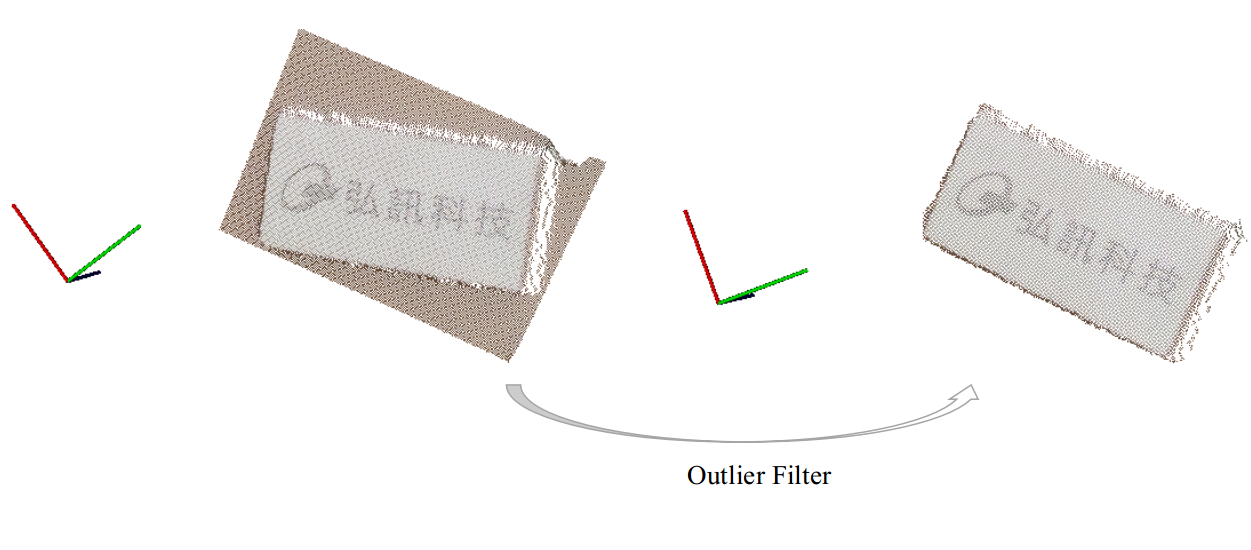
\includegraphics[width=13cm]{outlier-filter}
  \caption{Outlier filter效果图}
  \label{fig:outlier-filter}
\end{figure}


\subsection{ICP算法}
ICP(Iterative Closest Point)算法,即最近点迭代算法,是最为经典的数据配准算法。ICP算法本质上是基于最小二乘法的最优配准方法。该算法重复进行选择对应关系点对,计算最优刚体变换,直到满足正确配准的收敛精度要求。由于ICP算法是一种迭代算法,因此只要时间允许便可以获取足够精度的解,但也正因为如此,ICP也容易陷入局部最优解。本文充分考虑了ICP算法的这个特点,通过Angle-fixed 4PCS算法给出初始的刚体变换来避免ICP算法陷入局部最优解,同时通过迭代来提高最后输出的刚体变换精度。下面介绍一下ICP算法的基本原理。

给定两个点集$P_n:=\left\{\mathbf{p}_1,\mathbf{p}_2,\ldots,\mathbf{p}_n\right\}$和$Q_m:=\left\{\mathbf{q}_1,\mathbf{q}_2,\ldots,\mathbf{q}_m\right\}$,以及初始旋转变换$R$和平移变换$t$,以及迭代结束额距离误差$\delta$,ICP算法迭代步骤如下:
\begin{itemize}
\item {\kai 步骤1:}根据当前$R$和$t$,对于点集$P_n$中的每个点在$Q_m$中找出距离最近的点,构成点集$Q_n$;
\item {\kai 步骤2:}计算$P_n$和$Q_n$之间的距离的均方根误差:
  \begin{equation}
    E(R,t) = \frac{1}{n}\sum_{i=1}^n{\parallel \mathbf{q}_i - R\mathbf{p}_i - t\parallel}
  \end{equation}
  通过奇异值分解求得使得$E(R,t)$最小的$R'$和$t'$;
\item {\kai 步骤3:}如果$E(R,t) < \delta$,结束迭代;否则$R\leftarrow R'$,$t\leftarrow t'$,跳转至步骤1。
\end{itemize}

ICP算法的迭代过程还是相对来说十分简单的,唯一需要思考一下的是如何求得最小化$E(R,t)$的$R'$和$t'$,通过奇异值分解求解$R'$和$t'$的方法如下:

首先,记
\begin{equation}
  \left\{
  \begin{array}{ccccc}
  P_n'& = &\left\{\mathbf{p}_i-\mathbf{\mu}_p \;|\; \forall \mathbf{p}_i \in P_n\right\}&:=&\left\{\mathbf{p}'_i\right\}\\
  Q_n'& = &\left\{\mathbf{q}_i-\mathbf{\mu}_q \;|\; \forall \mathbf{q}_i \in Q_n\right\}&:=&\left\{\mathbf{q}'_i\right\}
  \end{array}
  \right.
\end{equation}
其中
\begin{equation}
  \left\{
    \begin{array}{ccc}
      \mathbf{\mu}_p&=&\frac{1}{n}\sum_{i=1}^n{\mathbf{p}_i}\\
      \mathbf{\mu}_q&=&\frac{1}{n}\sum_{i=1}^n{\mathbf{q}_i}
    \end{array}
  \right.
\end{equation}
再另
\begin{equation}
  W = \sum_{i=1}^n{\mathbf{p}_i'\mathbf{q}_i'}
\end{equation}
然后对矩阵$W$进行奇异值分解:
\begin{equation}
  W = U\Sigma V^T
\end{equation}
则
\begin{equation}
  \left\{
    \begin{array}{ccc}
      R'&=&UV^T \\
        t'&=&\mathbf{\mu}_p-R'\mathbf{\mu}_q
    \end{array}
    \right.
\end{equation}

\section{点云匹配实验}
为了评价所设计的算法A4PCS-ICP,考察其匹配精度以及时间性能,本文设计了位姿估计的实验,不但考察了A4PCS-ICP的性能,还与其他一些算法作比较,验证了A4PCS-ICP算法的匹配的精确度。

\subsection{实验内容}
实验在多了点云匹配的数据集上测试了A4PCS-ICP算法和一个基于局部特征描述子和RANSAC的算法LD-RANSAC\cite{li2005multiscale}。数据集中的点云数据有从激光扫描获取的、深度摄像头采集的、双目摄像头重构的,并且里面的模型也多种多样,有人造物、纹理缺少的物体,光滑的物体,粗糙的物体等。与A4PCS-ICP对比的LD-RANSAC算法使用了基于spin-image的描述子\cite{johnson1999using},LD-RANSAC的具体实现直接使用了PCL(Point Cloud Library)中的相关代码,人工配置了算法的参数以达到较好的匹配效果。

实验主要考察点云匹配的误差以及算法的运行时间,点云匹配的误差定义为两个点云之间的RMS误差:
\begin{equation}
  S = \sqrt{\frac{1}{N}\sum_{i=1}^{N}{\min_{p_j\in T(P')}\norm{q_i-p_j}^2}}
\end{equation}
显然RMS误差越小,点云的匹配效果越好,精度越高。

\subsection{实验结果}
为了考察算法的精度,通过对输入数据增加高斯噪声,来观察算法在不同大小噪声下的RMS误差,A4PCS-ICP算法和LD-RANSAC算的RMS误差随高斯噪声方差的变化曲线如图\ref{fig:err-noise}所示。
\begin{figure}[ht]
  \centering
  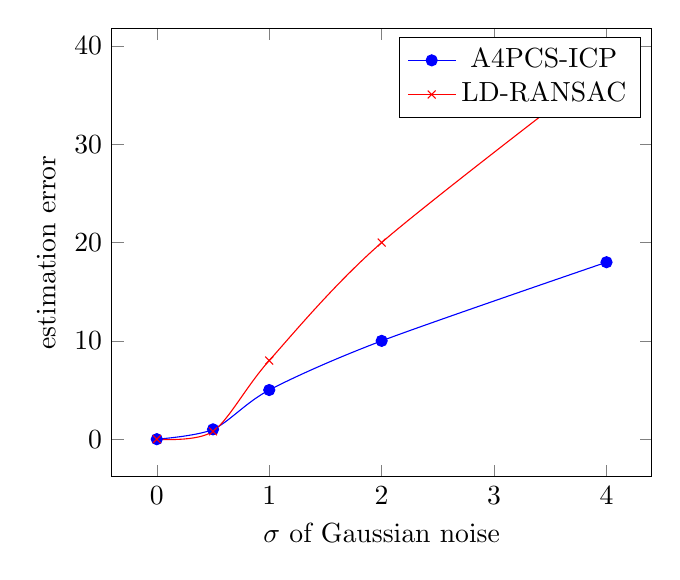
\begin{tikzpicture}
    \begin{axis}[xlabel=$\sigma$ of Gaussian noise, ylabel=estimation error]
      \addplot[smooth, mark=*, blue] plot coordinates {
        (0, 0)
        (0.5,1)
        (1, 5)
        (2, 10)
        (4, 18)
      };
      \addlegendentry{A4PCS-ICP}
      \addplot[smooth, mark=x, red] plot coordinates {
        (0, 0)
        (0.5,0.8)
        (1, 8)
        (2, 20)
        (4, 38)
      };
      \addlegendentry{LD-RANSAC}
    \end{axis}
  \end{tikzpicture}
  \caption{匹配误差随噪声变化曲线}
  \label{fig:err-noise}
\end{figure}
图中可以看出A4PS-ICP比LD-RANSAC算法有更小的误差,并且A4PCS-ICP对噪声也具有高强的鲁棒性。

为了考察算法的时间性能,通过对输入数据进行降采样(uniform sampling),变化uniform sampling的采集间距来变化输入点云的数量大小,不同点云数量大小下算法的运算时间的变化曲线如图\ref{fig:time-size}所示。
\begin{figure}[ht]
  \centering
  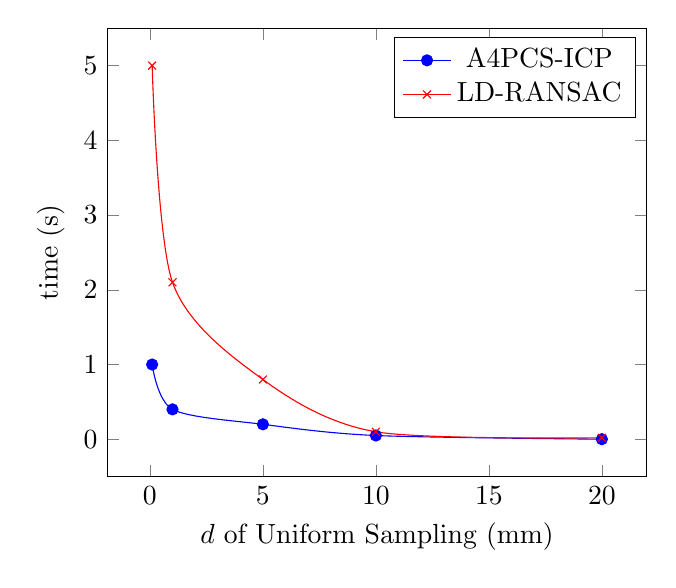
\begin{tikzpicture}
    \begin{axis}[xlabel=$d$ of Uniform Sampling (mm), ylabel=time (s)]
      \addplot[smooth, mark=*, blue] plot coordinates {
        (0.1, 1)
        (1,0.4)
        (5, 0.2)
        (10, 0.05)
        (20, 0.001)
      };
      \addlegendentry{A4PCS-ICP}
      \addplot[smooth, mark=x, red] plot coordinates {
        (0.1, 5)
        (1,2.1)
        (5, 0.8)
        (10, 0.1)
        (20, 0.02)
      };
      \addlegendentry{LD-RANSAC}
    \end{axis}
  \end{tikzpicture}
  \caption{匹配时间随点云数量大小变化曲线}
  \label{fig:time-size}
\end{figure}
图中可以看出A4PCS-ICP的运算时间比LD-RANSAC少,并且随着点云数量的增加其运算时间的差距越来越大。

综上,A4PCS-ICP算法相比LD-RANSAC算法具有更高的匹配精度,对噪声的鲁棒性也更强,并且算法的时间复杂度也更小。

\section{本章小结}
本章在4PCS算法的基础上,针对其缺点,提出了A4PCS算法,减少了算法的运算时间;然后为了提高匹配精度,将A4PCS算法与ICP算法相结合构成A4PCS-ICP算法。最后通过实验与LD-RANSAC算法相比较,实验表明A4PCS-ICP算法相比LD-RANSAC算法具有更高的匹配精度,对噪声的鲁棒性也更强,并且算法的时间复杂度也更小。


%%% Local Variables:
%%% TeX-master: "../thesis.tex"
%%% End: